%%% ML: poznamce pod carou v nazvu kapitoly by bylo dobre se vyhnout
%%% (ikonku premistit dal do textu a pod)
\chapter[Zásuvný modul]{Zásuvný
modul 
\includegraphics[scale=0.65]{./pictures/ikonka.png}\footnote{Zdroj:
SÚRO, v.v.i.}}
\label{4-plugin}

V~následujícím textu bude popsán postup tvorby nového softwarového
nástroje \textit{Ground radiation monitoring} a jeho
funkcionalita. Při vývoji nástroje bylo čerpáno z~doporučené
literatury \cite{masteringQgis} \cite{diveIntoPython} \cite{rapidPyQt}.

\section{Zadání} Zadáním bakalářské práce bylo vytvoření softwarového
nástroje, který ze vstupní interpolované mapy dávkových příkonů
extrahuje data do naplánovaných tras moni\-torování a vypočítá obdrženou
dávku záření gama při zadané rychlosti. Nástroj dále vypočte
jednoduché statistiky, maximální a průměrný dávkový příkon, délku
trasy, čas a kumulativní dávku v~určitých zadaných intervalech.

\subsection{Vstupní data}
\label{subsec:vstupniData}
\begin{enumerate}
	\item \textbf{Interpolovaná mapa dávkového příkonu} \\ Mapa je
v~souřadnicovém systému WGS84 EPSG:4326. Je vytvořena v~rastrovém
formátu, který je podporován knihovnou
GDAL\footnote{\url{http://www.gdal.org/formats\_list.html}}. Obsahuje
hodnoty dávkového příkonu v~daných jednotkách. (Plugin umožňuje volit
typ jednotek).
	\item \textbf{Trasa monitorování} \\ Trasa monitorování je
taktéž v~souřadnicovém systému WGS84 EPSG:4326. Je vytvořena ve
vektorovém formátu, který je podporován knihovnou
OGR\footnote{\url{http://www.gdal.org/ogr\_formats.html}}. Trasy mohou být
generované pomocí plánovačů tras (např. společnosti Google, Inc.)
\end{enumerate}

\begin{figure}[H] \centering
    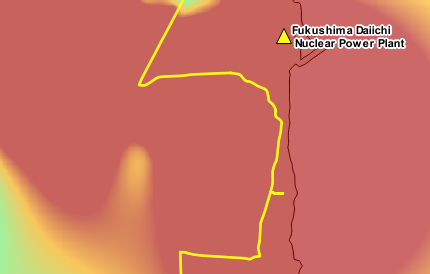
\includegraphics[scale=0.6]{./pictures/ukazka_vstupnich_dat.png}
    \caption[Ukázka vstupních dat]{Ukázka vstupních dat (zdroj:
vlastní, data poskytnutá od SÚRO, v.v.i.)}
    \label{fig:vstup}
\end{figure}
  			
\subsection{Výstupní data}
\label{sec:VystupniData}
\begin{enumerate}
	\item \textbf{Soubor se zprávou o~výpočtu} \\ Soubor se
zprávou o~výpočtu v~textovém formátu (\textit{.txt}) obsahuje
následující informace o~výpočtu (v~anglickém jazyce):
		\begin{itemize}
			\item čas vytvoření zprávy (\textit{report
created})
			
			\item informace o~trase (\textit{route
information})
			\begin{itemize}
				\item název trasy (\textit{route})
				\item zadaná rychlost v~km/h
(\textit{monitoring speed (km/h)})
				\item celkový čas monitorování
v~h:mm:ss (\textit{total monitoring time (h:mm:ss)})
				\item celková vzdálenost v~km
(\textit{total distance (km)})
			\end{itemize}
			
			\item informace o~části trasy bez dostupných
dat (v~místech, kde trasa přesahuje mapu dávkového příkonu)
(\textit{no data})
			\begin{itemize}
				\item čas (\textit{time})
				\item vzdálenost v~km
(\textit{distance (km)})
			\end{itemize}
			
			\item statistické hodnoty (\textit{radiation
values (estimated)})
			\begin{itemize}
				\item maximální dávkový příkon
v~$\mu$Sv/h (\textit{maximum dose rate ($\mu$Sv/h)})
				\item průměrný dávkový příkon
v~$\mu$Sv/h (\textit{average dose rate ($\mu$Sv/h)})
				\item celková dávka v~$\mu$Sv
(\textit{total dose ($\mu$Sv)})
			\end{itemize}
			
			\item nastavení (\textit{plugin settings})
			\begin{itemize}
				\item jednotky dávkového příkonu
vstupní mapy (\textit{input raster units})
				\item vzdálenost mezi body
navzorkované trasy v~m (vysvětleno v~kapitole
\ref{subsec:vzorkovaniLinie} (\textit{distance between track vertices
(m)})
			\end{itemize}
			
		\end{itemize}
Ukázku zprávy o výpočtu lze nalézt v obrázku \ref{fig:report}.	
			\begin{figure}[H] \centering
      			
\includegraphics[scale=0.9]{./pictures/report.png}
      				\caption[Ukázka zprávy
o~výpočtu]{Ukázka zprávy o~výpočtu (zdroj: vlastní)}
     				\label{fig:report}
  			\end{figure}
  			
	\item \textbf{Soubor trasy} \\ Soubor trasy obsahuje bodovou
vrstvu ve formátu Esri Shapefile (\textit{.shp}) s~body trasy
navzorkované dle zadání uživatele (vysvětleno v~kapitole
\ref{subsec:vzorkovaniLinie}) s~následujícími atributy (obr. \ref{fig:atributova_tabulka})
		\begin{itemize}
			\item dávkový příkon (\textit{rate uSvh})
			\item kumulativní čas (\textit{accTime})
			\item časový interval mezi body (\textit{interval s})
			\item kumulativní dávka (\textit{accDose})
		\end{itemize}
			\begin{figure}[H] \centering
      			
\includegraphics[scale=1]{./pictures/atributova_tabulka.png}
      				\caption[Výřez atributové
tabulky]{Výřez atributové tabulky (zdroj: vlastní)}
     				\label{fig:atributova_tabulka}
  			\end{figure}
  	
  	\item \textbf{Soubor s~údaji o~trase (volitelné)} \\ V~souboru
s~údaji o~trase ve formátu \zk{CSV} (\textit{.csv}) (obr. \ref{fig:csv}) jsou obsaženy
stejné hodnoty jako v~atributové tabulce navzorkované trasy. Navíc
soubor obsahuje souřadnice bodů. Vytvoření souboru je volitelné.
  			\begin{figure}[H] \centering
      			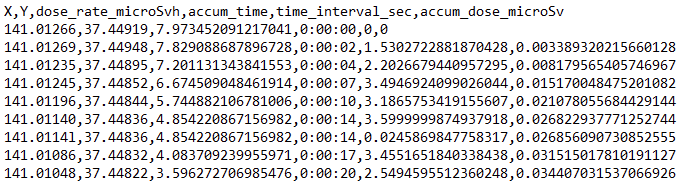
\includegraphics[scale=0.8]{./pictures/csv.png}
      				\caption[Výřez ze souboru s~hodnotami
oddělenými čárkou]{Výřez ze souboru s~hodnotami oddělenými čárkou
(zdroj: vlastní)}
     				\label{fig:csv}
  			\end{figure}
\end{enumerate}

\section{Kostra zásuvného modulu}
\subsection[Plugin Builder]{Plugin
Builder 
\includegraphics[scale=0.1]{./pictures/plugin_builder.png}}
K~vytvoření základu softwarového nástroje byl použit zásuvný modul
Plugin Builder dostupný z~oficiálního QGIS
repozitáře.\footnote{Dostupné
z~\url{https://plugins.qgis.org/plugins/pluginbuilder/}} Tento modul
pochází z~dílny organizace GeoApt LLC, jež se zabývá volně šiřitelnými
GIS. Po zadání základních informací (název modulu, základní popis,
autor, požadovaná verze QGIS, odkazy a další údaje o~repozitáři apod.)
vytvoří Plugin Builder kostru nového zásuvného modulu. Tato kostra
zajišťuje základní funkcionalitu modulu, tedy zobrazení a vypnutí okna
nebo také tlačítka \texttt{OK | Cancel}, pokud okno zásuvného modulu
není nastaveno jako "přichycovací".

\subsection{Popis souborů} Celý zásuvný modul \textit{Ground radiation
monitoring} se skládá z~několika souborů dohromady tvořících balíček,
který zajišťuje spustitelnost a funkcionalitu modulu. Některé soubory
zde budou dále prezentovány. Funkcionalita zásuvného modulu
zajišťující řešení zadání bakalářské práce je implementována v~posledních
dvou souborech následujícího výčtu.

\begin{itemize}
	\item \textbf{\_\_init\_\_.py} \\ Soubor slouží pro základní
inicializaci modulu.
		 
	\item \textbf{metadata.txt} \\ Tento textový soubor obsahuje
informace o~zásuvném modulu čtené Správcem zásuvných modulů. Vedle
údajů jako je jméno autora a název modulu je zde napří\-klad také údaj
o~požadované verzi QGIS, pro kterou je modul naprogramován. Správce
pak tento údaj porovná s~verzí QGIS a pokud dojde ke konfliktu, vypíše
chybovou hlášku a modul nenaimportuje.
	
	\item \textbf{Makefile} \\ V~souboru se nachází set instrukcí
např. pro zkompilování dokumentace nebo souboru \textbf{resources.qrc}
(zkompilovaná verze je \textbf{resources.py}), který informuje Qt jak
naložit s~ikonou modulu.
		
	\item \textbf{plugin\_upload.py} \\ Tento soubor slouží pro
nahrání modulu do QGIS repozitáře zásuvných modulů.

	\item \textbf{ground\_radiation\_monitoring.py} \\ Soubor
slouží pro implementaci zásuvného modulu do prostředí QGIS. Obsahuje
třídu \texttt{GroundRadiationMonitoring}. Zásadními metodami této
třídy jsou \texttt{add\_action} - metoda načítající ikonu modulu
(včetně názvu) do nástrojové lišty QGIS a~do~menu (přidává tedy
tlačítko na spuštění) a dále jsou to metody \texttt{onClosePlugin} a
\texttt{unload}, které se starají o~destrukci modulu.

	\item \textbf{ground\_radiation\_monitoring\_dockwidget.py} \\
Soubor zajišťuje propojení s~grafickým rozhraním, které je vytvořené
v~souboru \textbf{ground\_radiation\_monitoring\_base.ui} pomocí
prostředí QT Designer. Obsahuje třídu
\texttt{GroundRadiationDockWidget}, ve které jsou implementovány metody
pro načítání vstupních dat, čtení údajů zadaných uživatelem a
především také pro spuštění (a případné přerušení) procesu výpočtu a
práci s~výstupním souborem trasy (pokud si to uživatel přeje, vrstva
s~trasou může být načtena do QGIS). V~případě chyby při zadání
vstupních parametrů (např. zadání textu do pole, do kterého má být
zadané číslo nebo výběr výstupního souboru, do kterého je zápis
zakázán) je uživatel upozorněn chybovým hlášením.
	
	\item \textbf{ground\_radiation\_monitoring\_computation.py}
\\ V~souboru probíhá samotný výpočet dle uživatelsky zadaných dat a
vstupních parametrů. Obsahuje třídu
\texttt{GroundRadiationMonitoringComputation}, která je implementována
jako samostatné výpočetní vlákno. Výhodou je, že výpočet probíhá na
pozadí, tedy že s~QGIS se dá pracovat dále nezávisle na probíhajícím
procesu, což je nezbytné vzhledem k~jeho někdy dlouhému trvání
(v~závislosti na vstupních proměnných). V~této třídě jsou vedle
výpočetních metod obsaženy také metody pro vytváření výstupních
souborů. Třída během výpočtu komunikuje s~hlavním vláknem (s~třídou
\texttt{GroundRadiationMonitoringDockWidget}). Přes signály informuje
o~postupu výpočtu, který je zobrazován v~ukazateli průběhu výpočtu.
	
\end{itemize}

\newpage
\section{Algoritmus} V~této části práce bude popsán algoritmus
kódu. Nejprve bude prezentováno jednoduché schéma výpočtu, poté budou
jednotlivé části rozebrány více dopodrobna.
\subsection{Schéma výpočtu}
\begin{figure}[H] \centering
    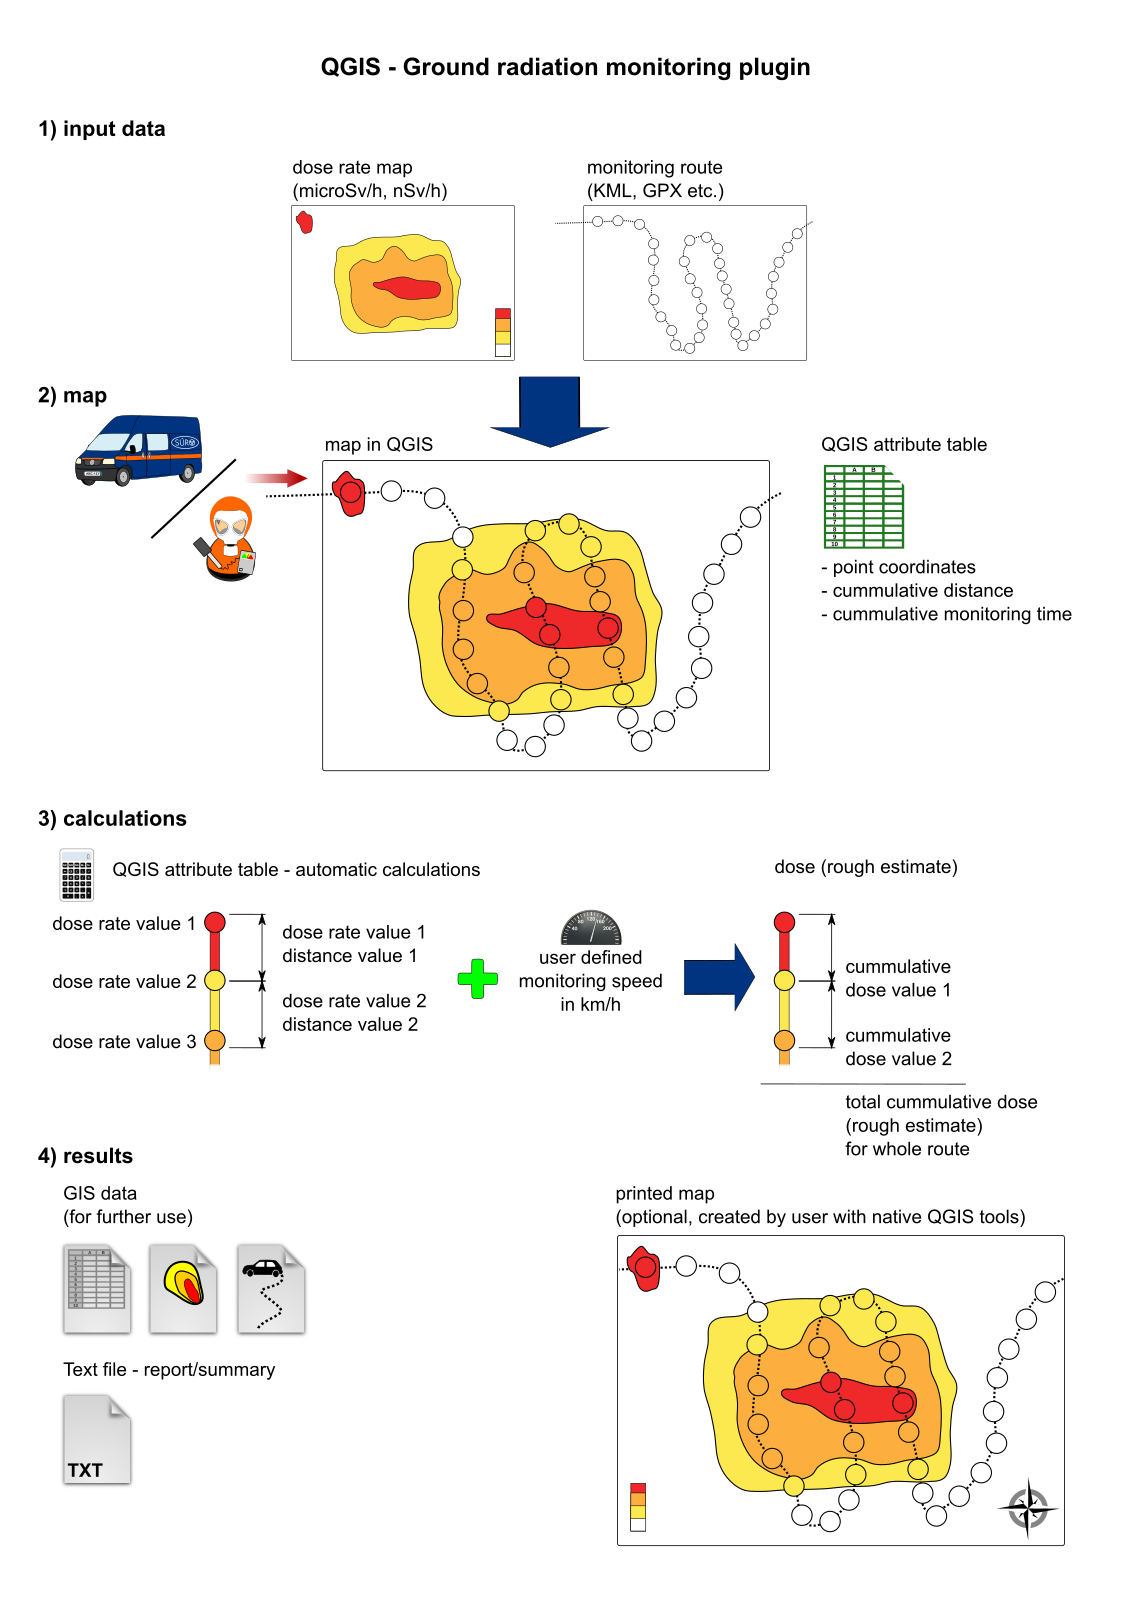
\includegraphics[scale=0.4]{./pictures/computation_scheme.png}
      	\caption[Schéma výpočtu]{Schéma výpočtu (zdroj: SÚRO, v.v.i.)}
    	\label{fig:SchemeOfComputation}
\end{figure}

Schéma výpočtu je zřejmé z~obrázku
\ref{fig:SchemeOfComputation}. Z~interpolované mapy dávkových příkonů
(\textit{dose rate map}) jsou extrahovány rastrové hodnoty
(\textit{dose rate value}) v~bodech navzorkované trasy
(\textit{monitoring route}). Dále jsou provedeny výpočty, tedy dle
vzdálenosti (\textit{distance value}) mezi jednotlivými body trasy a
zadané rychlosti (\textit{user defined monitoring speed}) je spočtena
obdržená dávka záření na daném úseku (\textit{cumullative)}. Rychlost
je konstantní pro celou trasu. Tyto hodnoty společně s~časy potřebnými
na projetí jednotlivých úseků jsou zapsány do atributové tabulky nově
vzniklé vrstvy a volitelně do \zk{CSV} souboru. Statistiky o~celé
trase, jak již bylo řečeno v~sekci \ref{sec:VystupniData}, jsou
uloženy do textového souboru se zprávou o~výpočtu.

\subsection{Vzorkování linie}
\label{subsec:vzorkovaniLinie} Vstupní trasa monitorování se skládá
z~několika přímých linií vzájemně propojených vrcholy. Délka
jednotlivých segmentů se odvíjí od přímosti úseků trasy. Např. pokud
součástí trasy bude dálnice s~přímým úsekem dlouhým 10 km, pak stejně
bude dlouhý i segment mezi vrcholy na začátku a konci tohoto
úseku. Jelikož snímání hodnot rastru probíhá na daných souřadnicích a
jediné známé souřadnice trasy jsou právě ty vrcholové, tak by bez
dalších úprav došlo k~hrubým chybám ve výpočtech resp. výsledky by
byly nesměrodatné. Je jasné, že kdyby uprostřed dlouhého rovného úseku
byla oblast se zvýšeným dávkovým příkonem, tak tato skutečnost by do
výpočtu nebyla vůbec zahrnuta (hodnoty rastru by byly sejmuté pouze na
koncích, tedy v~místech, která nenesou žádnou informaci o~zbytku
segmentu).

Z~tohoto důvodu je třeba trasu tzv. navzorkovat, tzn. rozdělit
jednotlivé rovné segmenty na více kratších částí. Takto dojde
k~získání souřadnic bodů, které mezi sebou budou mít kratší
vzdálenosti. Do výpočtu bude tak zahrnuto více informací o~dávkových
příkonech v~průběhu trasy a výsledek bude lépe odpovídat
skutečnosti. (Stále se však vzhledem k~jednoduchosti výpočtu bude
jednat pouze o~odhad).

Některé segmenty mohou být kratší, než uživatelsky zadaná vzorkovací
vzdálenost. Následující pseudokód
\ref{alg:getTrackVertices} popisuje algoritmus \texttt{Získání
souřadnic bodů trasy} (ve třídě
\texttt{GroundRadiationMonitoringComputation} jako metoda
\texttt{getTrackVertices}), který získává souřadnice vrcholů trasy a
na základě výpočtu vzdálenosti rozhoduje, zdali je potřeba trasu
v~jednotlivých segmentech navzorkovat. Pokud ano, segment je ihned
navzorkován zavoláním \texttt{navzorkujLinii} (ve třídě \\
\texttt{GroundRadiationMonitoringComputation} jako metoda
\texttt{sampleLine}). Výstupem algoritmu pro získání souřadnic je
dvourozměrné pole obsahující souřadnice bodů již navzorkované
linie. Vzdálenost mezi body je vypočtena pomocí QGIS třídy
\texttt{QgsDistanceArea}\footnote{\url{https://qgis.org/api/classQgsDistanceArea.html}}
a jejích metod, výpočet je proveden na referenčním elipsoidu
\textit{WGS84}. Extrahování souřadnic vrcholů trasy je provedeno
pomocí QGIS třídy
\texttt{QgsVectorLayer}\footnote{\url{https://qgis.org/api/classQgsVectorLayer.html}}
a její metody \texttt{getFeatures}.

\begin{algorithm}
\caption{Získání souřadnic bodů trasy}
\label{alg:getTrackVertices}
    \begin{algorithmic}[1] \STATE{\textbf{funkce} získejSouřadnice}
\STATE{extrahuj souřadnice vrcholů trasy do poleSouřadniceVrcholů}
\STATE{přidej poleSouřadniceVrcholů[0] do poleNovéSouřadnice} \FOR{i =
řada od 0 do (délka(poleSouřadniceVrcholů) - 2)} \STATE{bod1 =
poleSouřadniceVrcholů[i]} \STATE{bod2 = poleSouřadniceVrcholů[i + 1]}
\STATE{vzdálenost = vypočtiVzdálenost(bod1, bod2)} \IF{vzdálenost >
vzorkovacíVzdálenost} \STATE{novéBody = navzorkujLinii(bod1, bod2)}
\STATE{přidej novéBody do poleNovéSouřadnice} \ELSE \STATE{přidej bod2
do poleNovéSouřadnice}
    		\ENDIF
    	\ENDFOR \STATE{\textbf{return} poleNovéSouřadnice}
    \end{algorithmic}
\end{algorithm}

Je zřejmé, že všechny nově vzniklé úseky trasy nemají stejnou
délku. Je to dané tím, že délka původních segmentů není většinou
dělitelná zadanou vzorkovací vzdáleností bez zbytku. Např. segment
o~délce 10 m při vzorkovací vzdálenosti 3~m bude rozdělen celkem na
čtyři části, z~toho tři budou o~délce 3~m a jeden o~délce 1
m. Následující pseudokód \ref{alg:sampleLine} popisující výpočetní
funkci souřadnic nových bodů tuto skutečnost zohledňuje a
ověřuje. Algoritmus vypočte souřadnice bodu, který zakončuje tu část
segmentu, která je dělitelná vzorkovací vzdáleností beze zbytku (pokud
nastane případ, že segment je dělitelný beze zbytku, tato část
algoritmu není vykonávána). Tento bod je poté považován za konečný bod
(v~pseudokódu jako \texttt{konečnýBod}) segmentu a nově vzniklý úsek
je rozdělen na stejně dlouhé části.

\begin{algorithm}
\caption{Výpočet souřadnic bodů}
\label{alg:sampleLine}
	\begin{algorithmic}[1] \STATE{\textbf{funkce} navzorkujLinii
(bod1, bod2)} \STATE{početNovéBody = $\lceil$délkaSegment /
vzorkovacíVzd$\rceil$} - 1 \IF{délkaSegment \textbf{mod} vzorkovacíVzd
$\neq$ 0} \STATE{nejkratšíSegment\% = (délkaSegment \textbf{mod}
vzorkovacíVzd) / délkaSegment} \STATE{konečnýBod = bod2 - (bod2 -
bod1) $\cdot$ nejkratšíSegment\%} \STATE{vektor = konečnýBod - bod1}
\ELSE \STATE{vektor = bod2 - bod1}
		\ENDIF \STATE{přírůstek = vektor / početNovéBody}
\FOR{i = řada od 1 do početNovéBody} \STATE{přidej (bod1 + i $\cdot$
přírůstek) do poleNovéBody}
		\ENDFOR \IF{konečnýBod existuje} \STATE{přidej
(konečnýBod) do poleNovéBody}
		\ENDIF \STATE{přidej bod2 do poleNovéBody}
\STATE{\textbf{return} poleNovéBody}
	\end{algorithmic}
\end{algorithm}

\subsection{Výpočet statistik}
\label{subsec:vypocetStatistik} Získané souřadnice bodů navzorkované
trasy dále vstupují do procesu výpočtu statistik, hlavního výstupu
nástroje. Algoritmus výpočtu popisuje pseudokód v příloze \textbf{A} 
(implementace algoritmu je ve třídě \texttt{GroundRadiationMonitoringComputation} jako metoda
\texttt{getStatistics}). Výpočtu předchází získání hodnot rastru na
bodech. To je provedeno pomocí QGIS třídy
\texttt{QgsDataProvider}\footnote{\url{https://qgis.org/api/classQgsDataProvider.html}}
a jejích metod (v~pseudokódu jako \texttt{získejHodnotu}). Pole se
souřadnicemi bodů navzorkované trasy je v~pseudokódu označeno jako
\texttt{poleBody}. Pro výpočet vzdálenosti mezi body je použita stejná
metoda jako v~pseudokódu~\ref{alg:getTrackVertices}. Do výpočtu dále
vstupuje uživatelsky zadaná rychlost pohybu, která je považována za
konstantní na celé trase. Výstupem algoritmu jsou celkové statistiky
(viz. sekce \ref{sec:VystupniData}): celková délka a čas projetí
trasy, délka a čas projetí trasy mimo mapu dávkových příkonů,
maximální a průměrný dávkový příkon na trase a celková dávka. Výstupem
jsou dále i dílčí statistiky na jednotlivých bodech trasy, které jsou
dále zapsány do atributové tabulky nově vzniklé vrstvy a případně i do
\zk{CSV} souboru (viz. sekce \ref{sec:VystupniData}). Data zapisovaná
do souborů vypovídající o~dávce a dávkovém příkonu jsou přenásobována
koeficientem podle zvolených jednotek mapy dávkového příkonu
uživatelem.




Může se stát, že trasa probíhá mimo mapu dávkových příkonů. Extrakce
hodnoty rastru v~bodě, který leží mimo něj, vrací hodnotu
\texttt{None}, tedy že data nejsou dostupná. Prezentovaný algoritmus
v~tomto případě místo None zapíše číslo 0. Podobně, pokud je hodnota
rastru menší než 0, algoritmus tuto hodnotu přepíše na 0. Do
výsledných statistik, jak již bylo zmíněno, jsou počítány délka a čas
projetí trasy mimo rastr, tj. když je hodnota rastru 0. Do průměrného
dávkového příkonu na trase nejsou tyto hodnoty započítávané.

%%% ML: pridal jsem tak, aby testovaci data zacinala az pod
%%% pseudokodem. Pseudokod je sam o sobe hodne dlouhy, skoro by patril
%%% do prilohy

%%% MK: Dal jsem ho do přílohy.

\section{Testovací data} Testování zásuvného modulu při vývoji
probíhalo s~využitím dat připravených od \zk{SÚRO}.

\subsection{Interpolovaná data dávkových příkonů} Pro tvorbu
interpolované mapy dávkových příkonů byla využita část reálných měření
projektu Safecast v~oblasti prefektury Fukushima (Japonsko). Měření
prováděly dobrovolnické mobilní skupiny a obsahují informace o~času
měření, GPS souřadnice a hodnoty dávkového příkonu záření gama
v~$\mu$Sv/h. Kompletní dataset je dostupný ke stažení ve formátu
\zk{CSV} na webových stránkách projektu. Dataset je uvolněn pod
licencí CC0 1.0 Universal (CC0 1.0) Public Domain
Dedication\footnote{\url{https://creativecommons.org/publicdomain/zero/1.0/}}.

Z~balíku dat byla vybrána zájmová oblast kolem jaderné elektrárny
Fukushima Daiichi. Data byla omezena pouze na měření z~roku
2011. V~open source programu
SAGA-GIS\footnote{\url{http://www.saga-gis.org}} byla z~dat
vytvořena interpolovaná mapa dávkových příkonů (obr. \ref{fig:interpolatedMap}) 
metodou Multilevel B-Spline
%%% ML: tento odkaz bych uz neuvadel. I tak je poznamek pod caru v textu uz prilis
%%% MK: smazáno
Interpolation.

\begin{figure}[H] \centering
    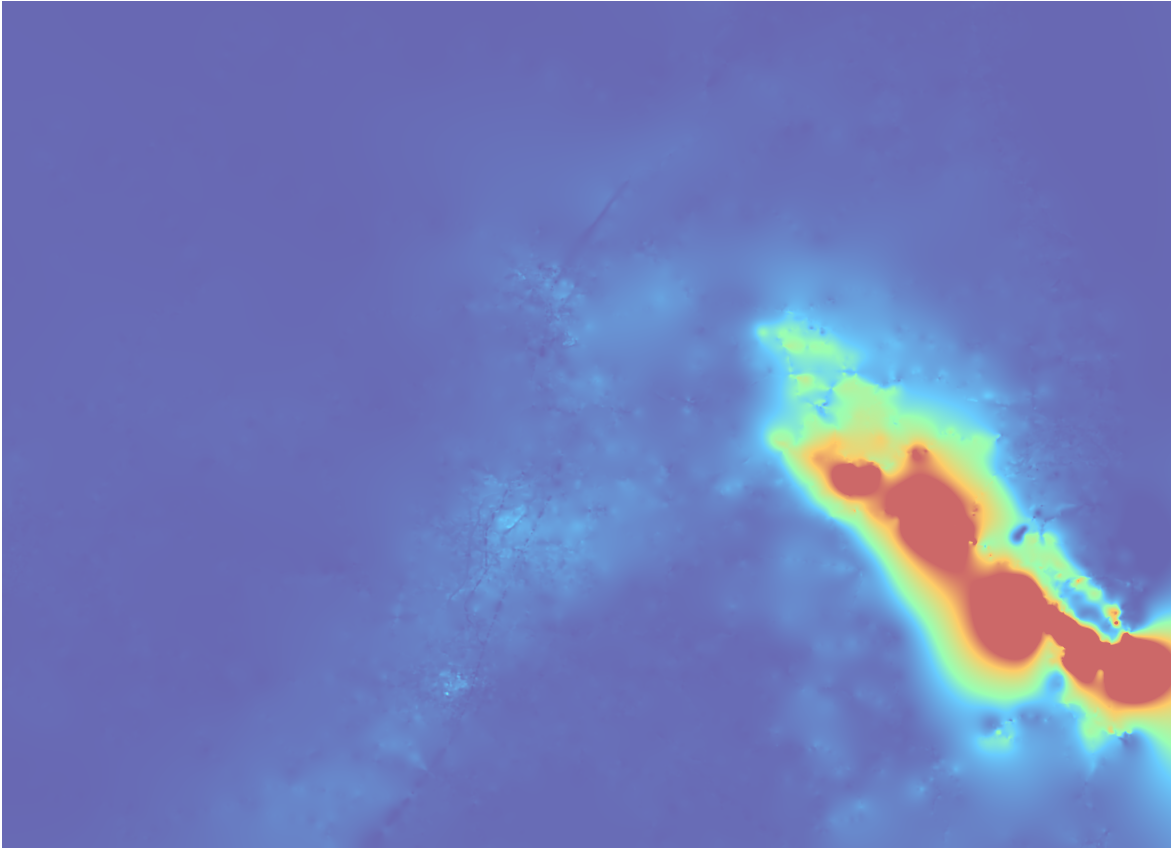
\includegraphics[scale=0.4]{./pictures/interpolovana_mapa.png}
      	\caption[Interpolovaná mapa dávkových příkonů (prefektura
Fukushima)]{Interpolovaná mapa dávkových příkonů gama záření
(prefektura Fukushima)}(zdroj: vlastní, data poskytnutá od SÚRO,
v.v.i.)
    	\label{fig:interpolatedMap}
\end{figure}

\subsection{Trasa monitorování} Trasy monitorování použité pro
testování byly naplánovány pomocí běžně používaných webových služeb
Mapy.cz a Google (jak již bylo zmíněno v~kapitole
\ref{subsec:vstupniData}). Trasy byly vyexportovány ve formátech
\zk{KML} a \zk{GPX}. Byly voleny tak, aby se jejich průběh co nejvíce
přiblížil \zk{JE} Fukushima a aby byla vidět výrazná změna hodnot
dávkových příkonů. Ukázku trasy monitorování lze nalézt v obr. \ref{fig:trasa}.
\newpage
\begin{figure}[H] \centering
    
\includegraphics[scale=0.3]{./pictures/trasa_monitorovani.png}
      	\caption[Trasa monitorování (Futaba-Nawashirogae, prefektura
Fukushima)]{Trasa monitorování (Futaba-Nawashirogae, prefektura
Fukushima)}(zdroj: vlastní, data poskytnutá od SÚRO, v.v.i.)
    	\label{fig:trasa}
\end{figure}

%%% ML: Chybi mi tu ukazky vystupu a zminka, ze vlastni navod na
%%% pouzit modulu je v priloze

%%% MK: Ukázky výstupu mám v podkapitole Výstupní data 

\section{Návod na použití}
K zásuvnému modulu byl vytvořen návod na použití v anglickém jazyce. 
Návod je uveden v příloze \textbf{B}. 